\chapter{Frontend Implementation}

\section{Overview}
The frontend of Nexora is built using HTML, CSS, and JavaScript, following a component-based architecture for better maintainability and reusability.

\section{Technologies Used}
\begin{itemize}
    \item HTML5 and CSS3
    \item JavaScript (ES6+)
    \item Bootstrap for responsive design
    \item jQuery for DOM manipulation
    \item AJAX for API communication
\end{itemize}

\section{Key Features}
\begin{itemize}
    \item Responsive Design:
    \begin{itemize}
        \item Mobile-first approach
        \item Cross-browser compatibility
        \item Intuitive navigation
        \item Modern UI components
    \end{itemize}
    \item User Experience:
    \begin{itemize}
        \item Fast page loading
        \item Smooth interactions
        \item Clear feedback
        \item Error handling
    \end{itemize}
    \item Integration with Backend:
    \begin{itemize}
        \item API calls for data retrieval
        \item Authentication and authorization
        \item Real-time updates
    \end{itemize}
\end{itemize}

\section{UI/UX}
% Add screenshots or diagrams here in logical order:
% Landing Page -> Authentication -> User -> Checkout -> Vendor -> Admin

% --- Landing Page ---
\begin{figure}[htbp]
\centering
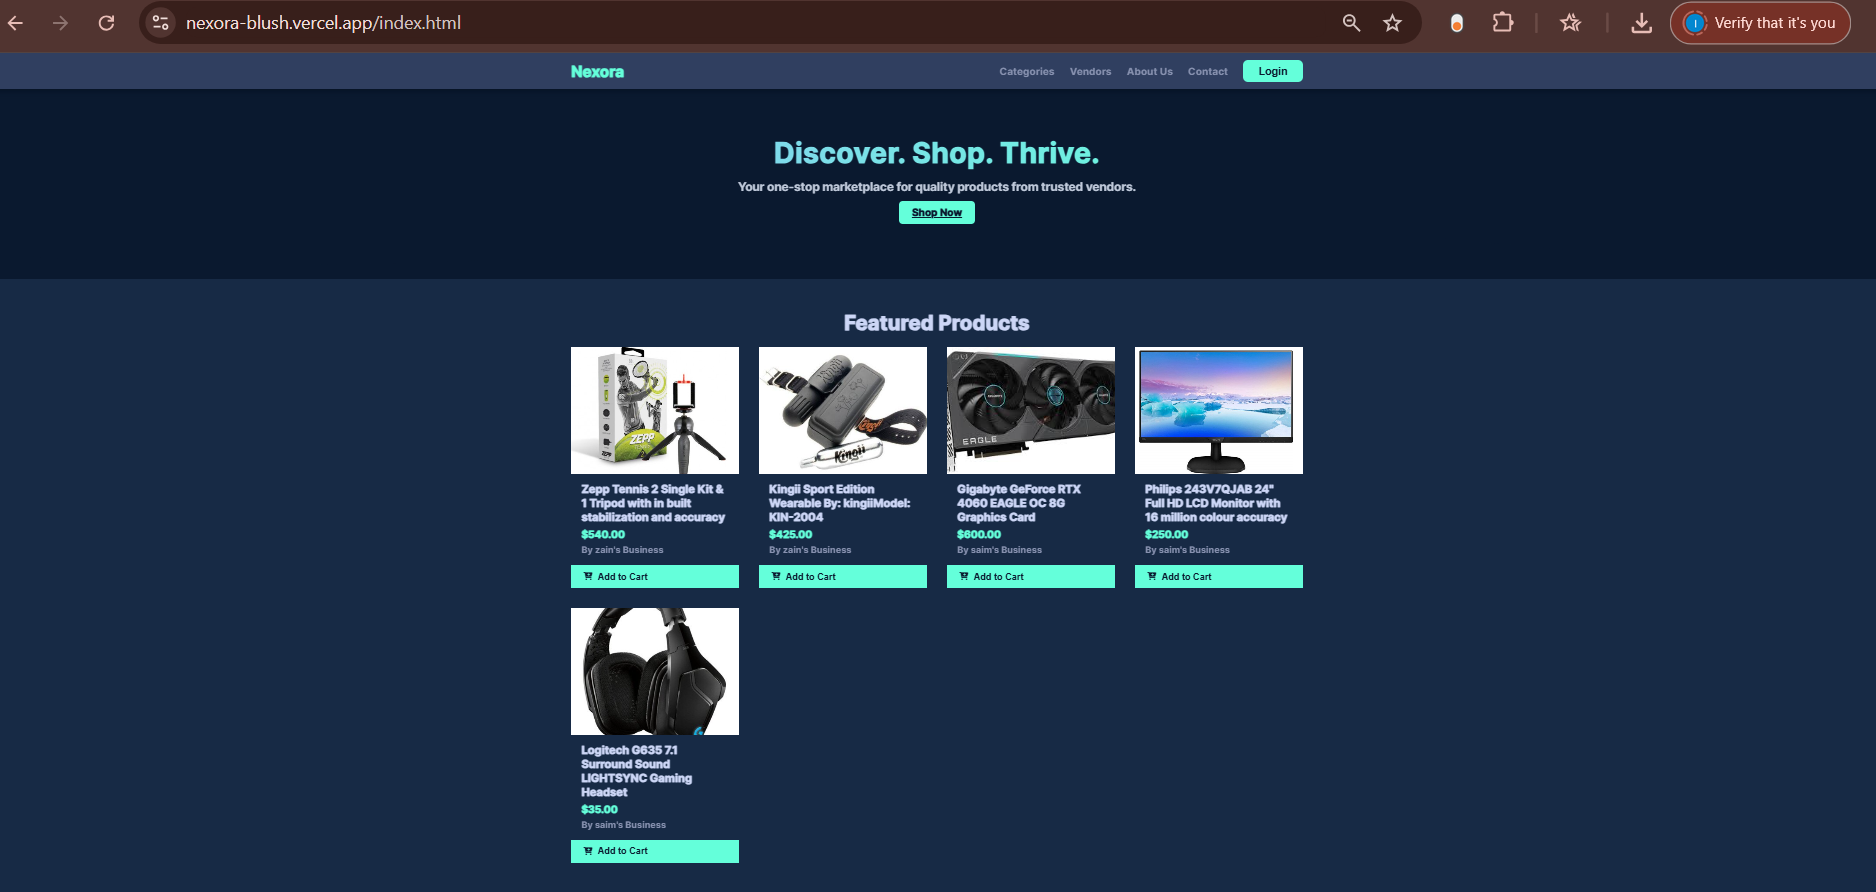
\includegraphics[width=\textwidth,keepaspectratio]{thesis/figures/Landing-Page.png}
\caption{Landing Page}
\label{fig:landing-page}
\end{figure}

% --- Authentication ---
\begin{figure}[htbp]
\centering
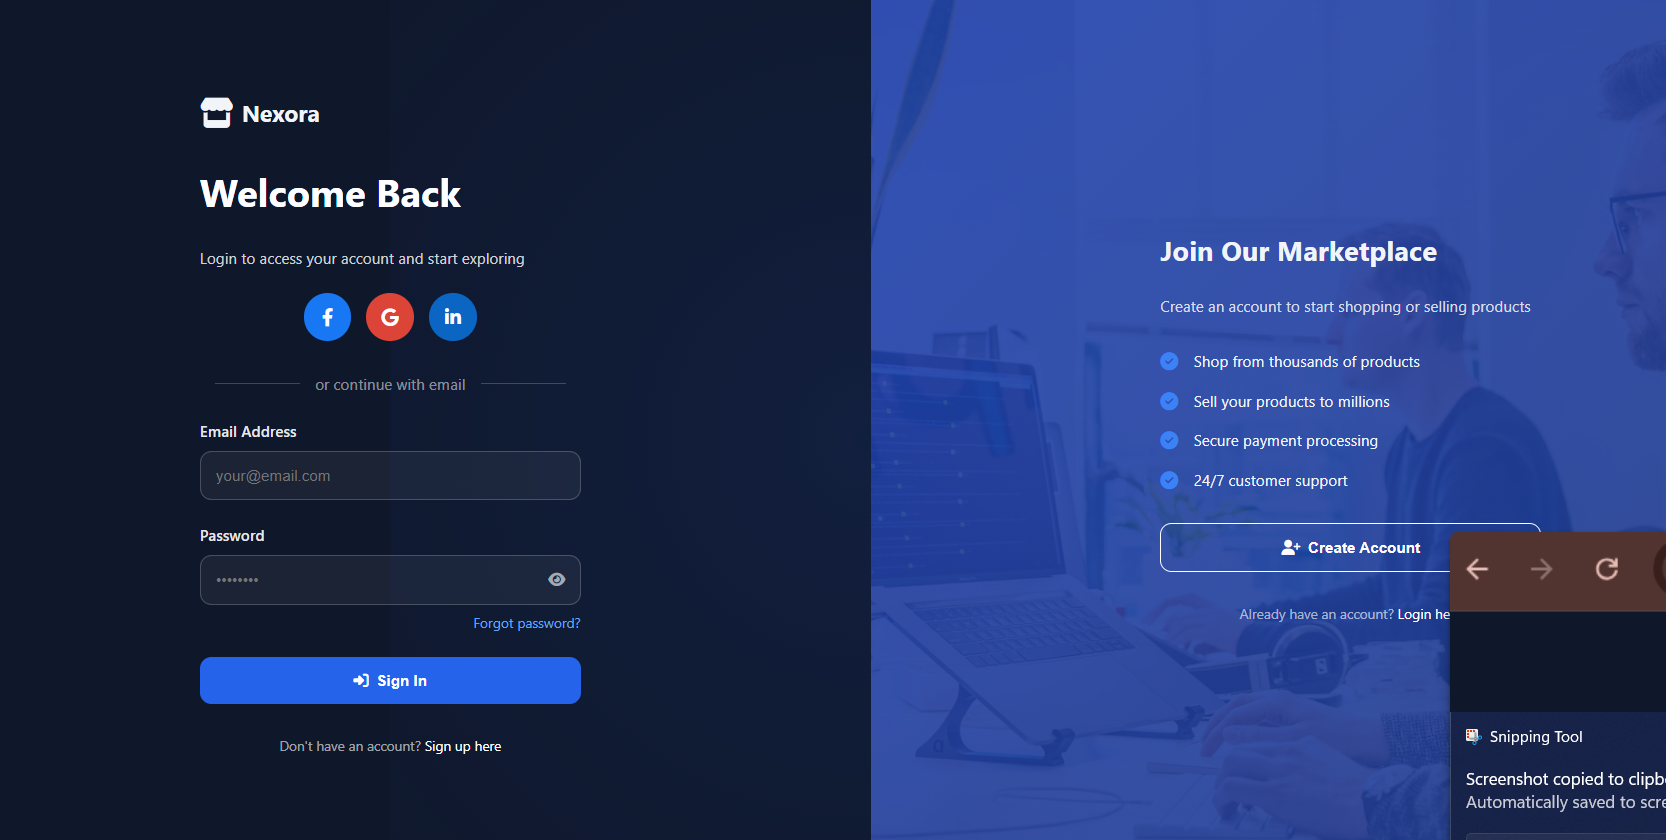
\includegraphics[width=\textwidth,keepaspectratio]{thesis/figures/Login-Registration.png}
\caption{Login and Registration Pages}
\label{fig:login-register}
\end{figure}

\begin{figure}[htbp]
\centering
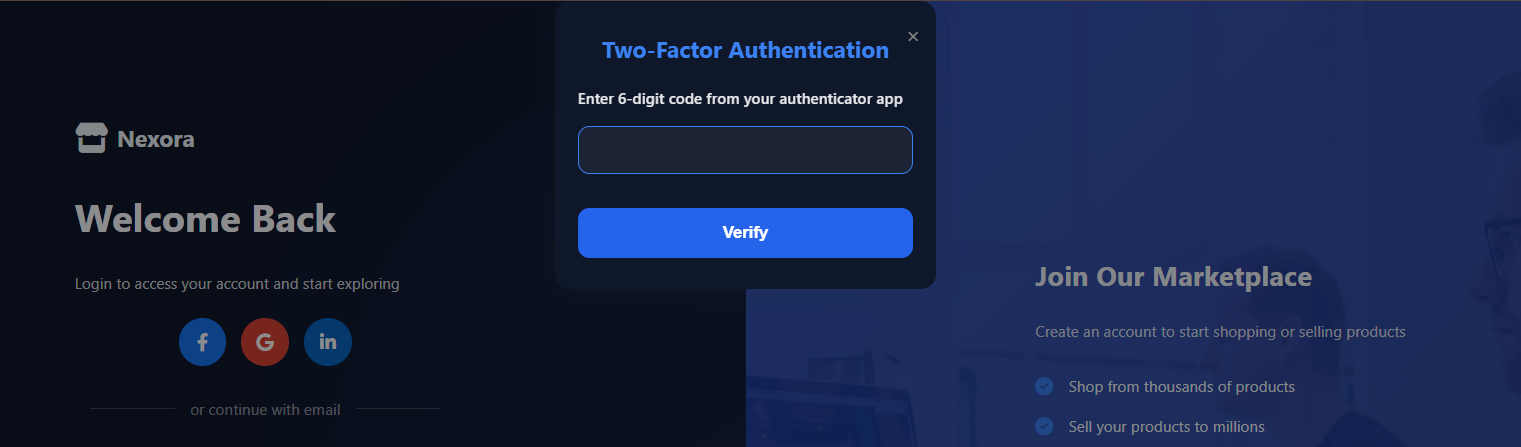
\includegraphics[width=\textwidth,keepaspectratio]{thesis/figures/2Fa.png}
\caption{2FA Authentication}
\label{fig:2fa}
\end{figure}

% --- User Interface ---
\begin{figure}[htbp]
\centering
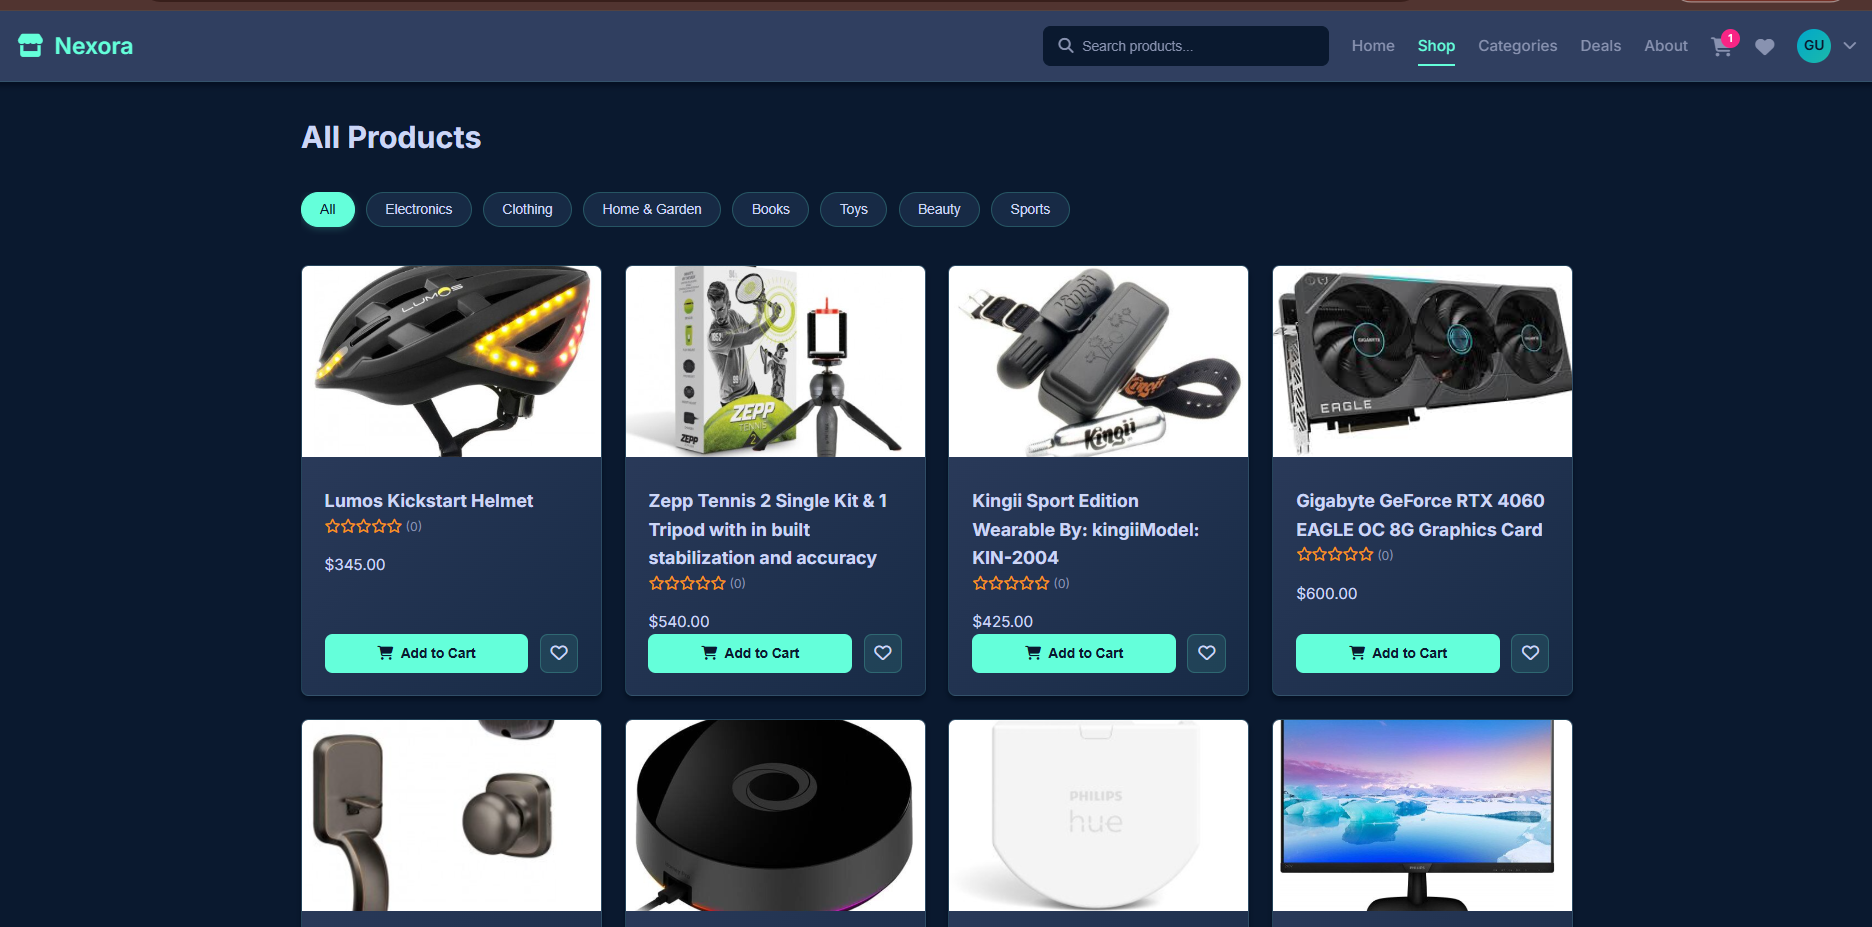
\includegraphics[width=\textwidth,keepaspectratio]{thesis/figures/User-Dashboard.png}
\caption{User Dashboard}
\label{fig:user-dashboard}
\end{figure}

\begin{figure}[htbp]
\centering
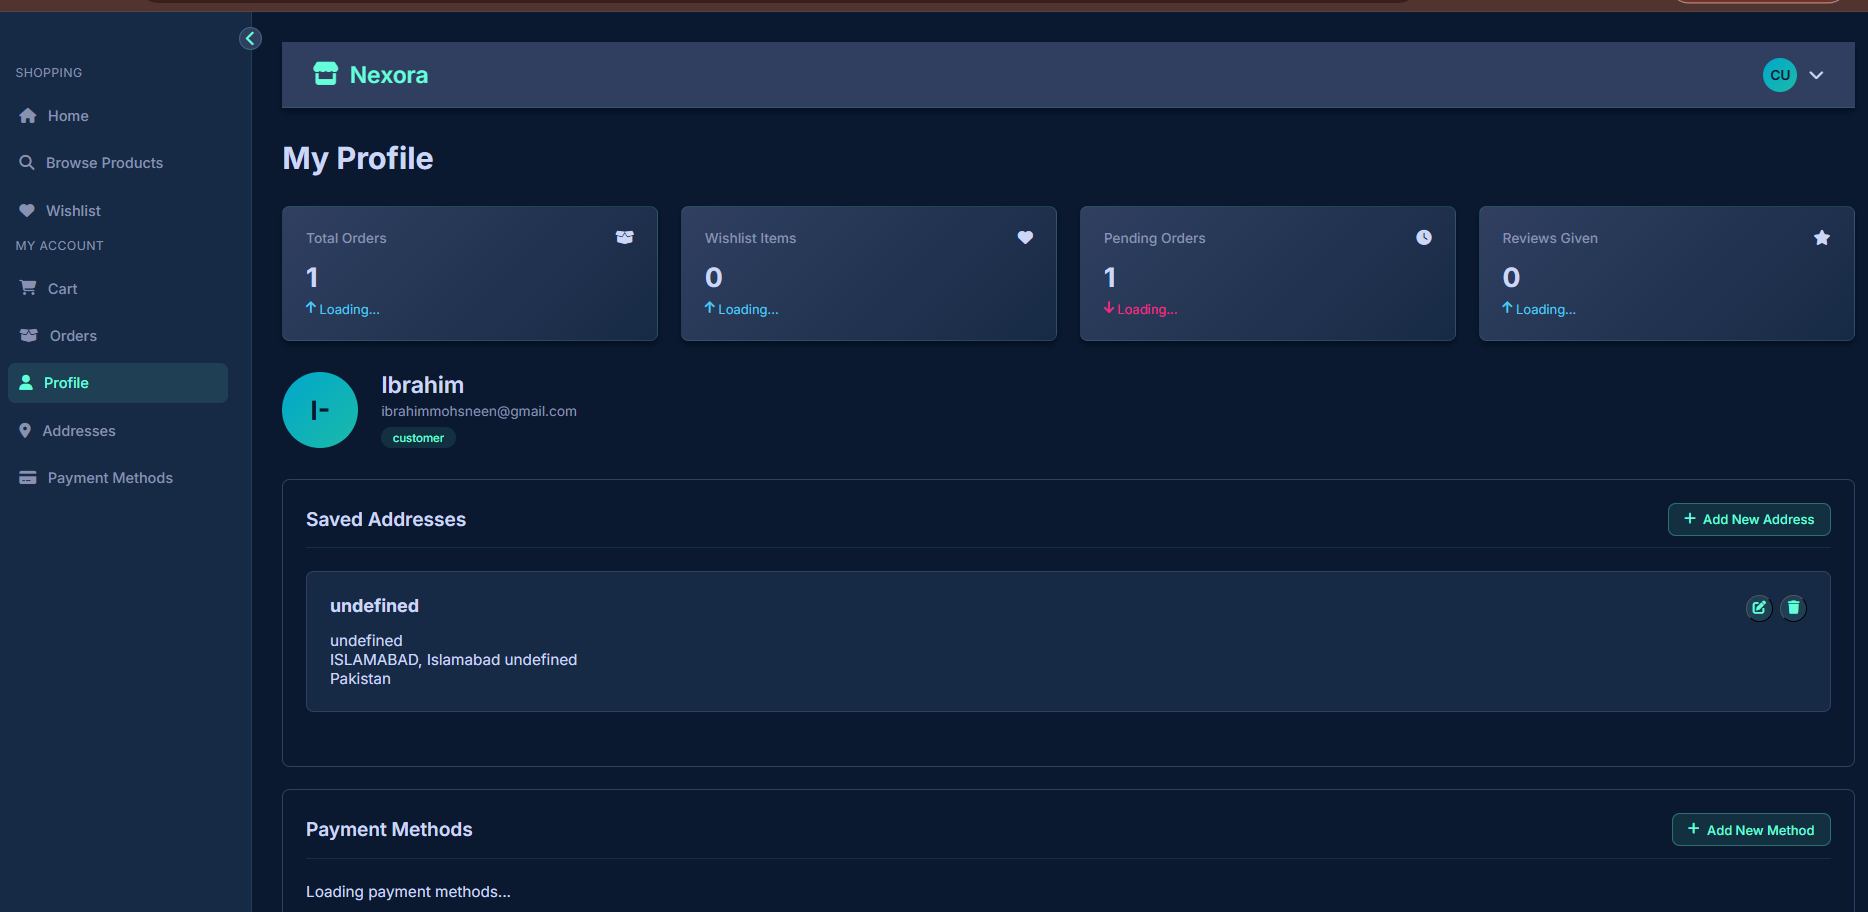
\includegraphics[width=\textwidth,keepaspectratio]{thesis/figures/User-Profile.png}
\caption{User Profile}
\label{fig:user-profile}
\end{figure}

% --- Checkout ---
\begin{figure}[htbp]
\centering
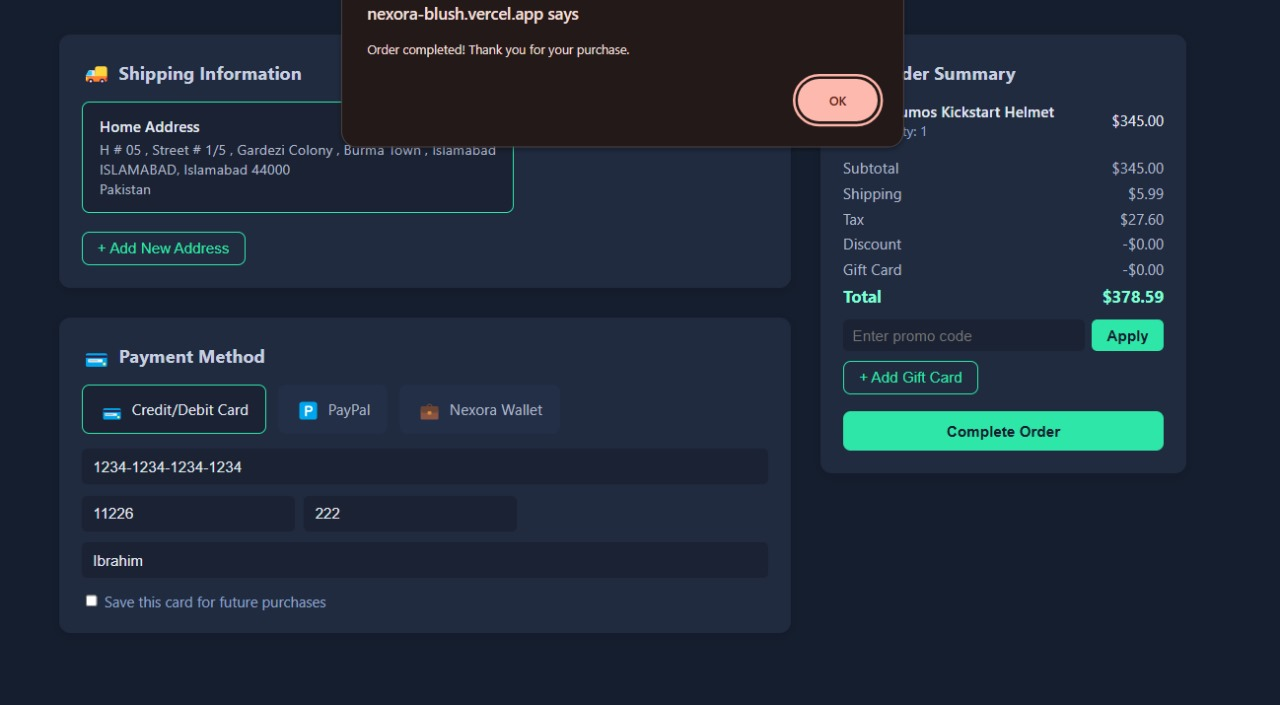
\includegraphics[width=\textwidth,keepaspectratio]{thesis/figures/Checkout.jpg}
\caption{Checkout Process}
\label{fig:checkout}
\end{figure}

% --- Vendor Interface ---
\begin{figure}[htbp]
\centering
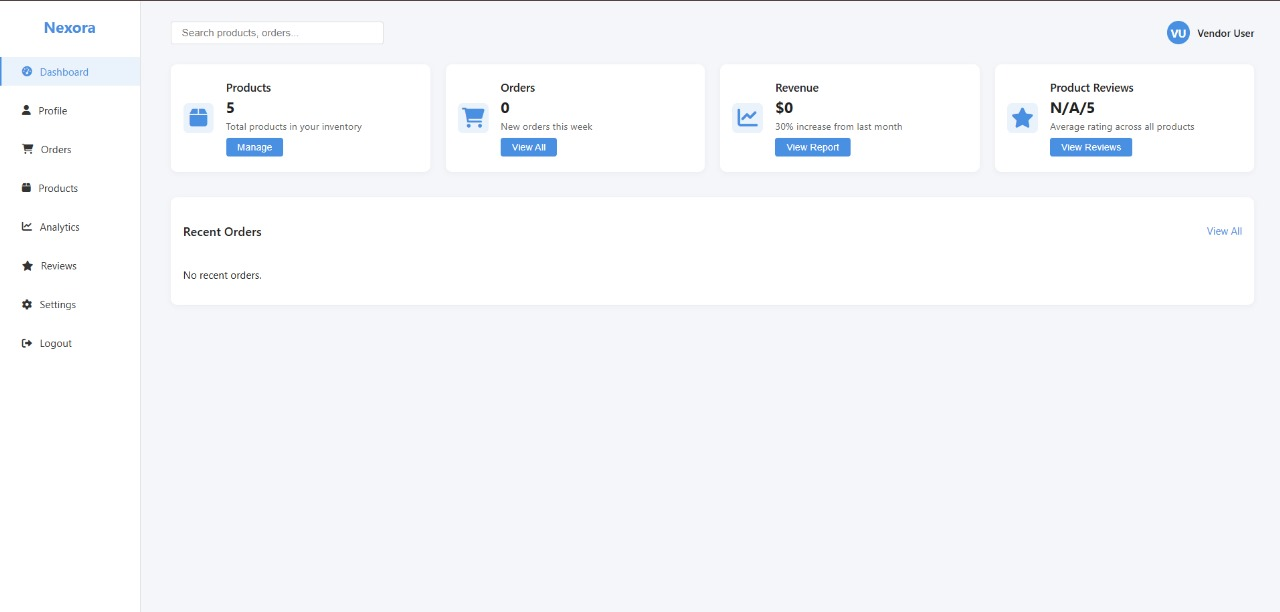
\includegraphics[width=\textwidth,keepaspectratio]{thesis/figures/Vendor-Dashboard.jpg}
\caption{Vendor Dashboard}
\label{fig:vendor-dashboard}
\end{figure}

\begin{figure}[htbp]
\centering
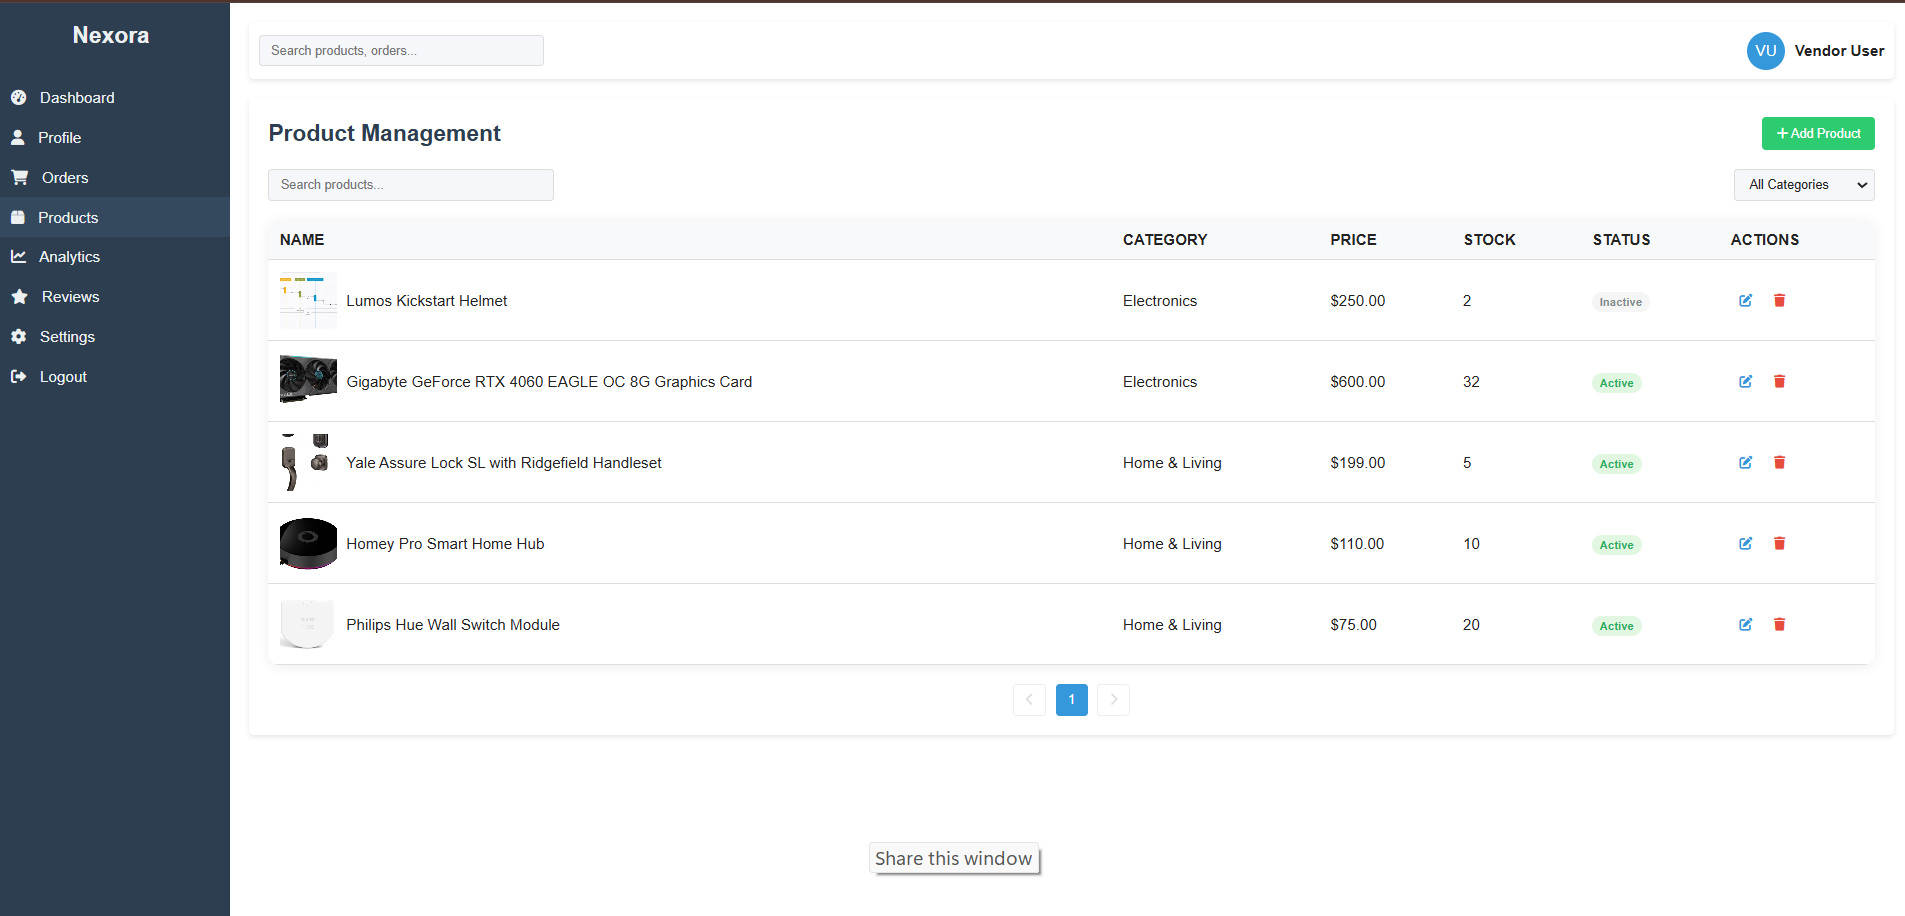
\includegraphics[width=\textwidth,keepaspectratio]{thesis/figures/Vendor-Products.png}
\caption{Vendor Product Management}
\label{fig:vendor-products}
\end{figure}

\begin{figure}[htbp]
\centering
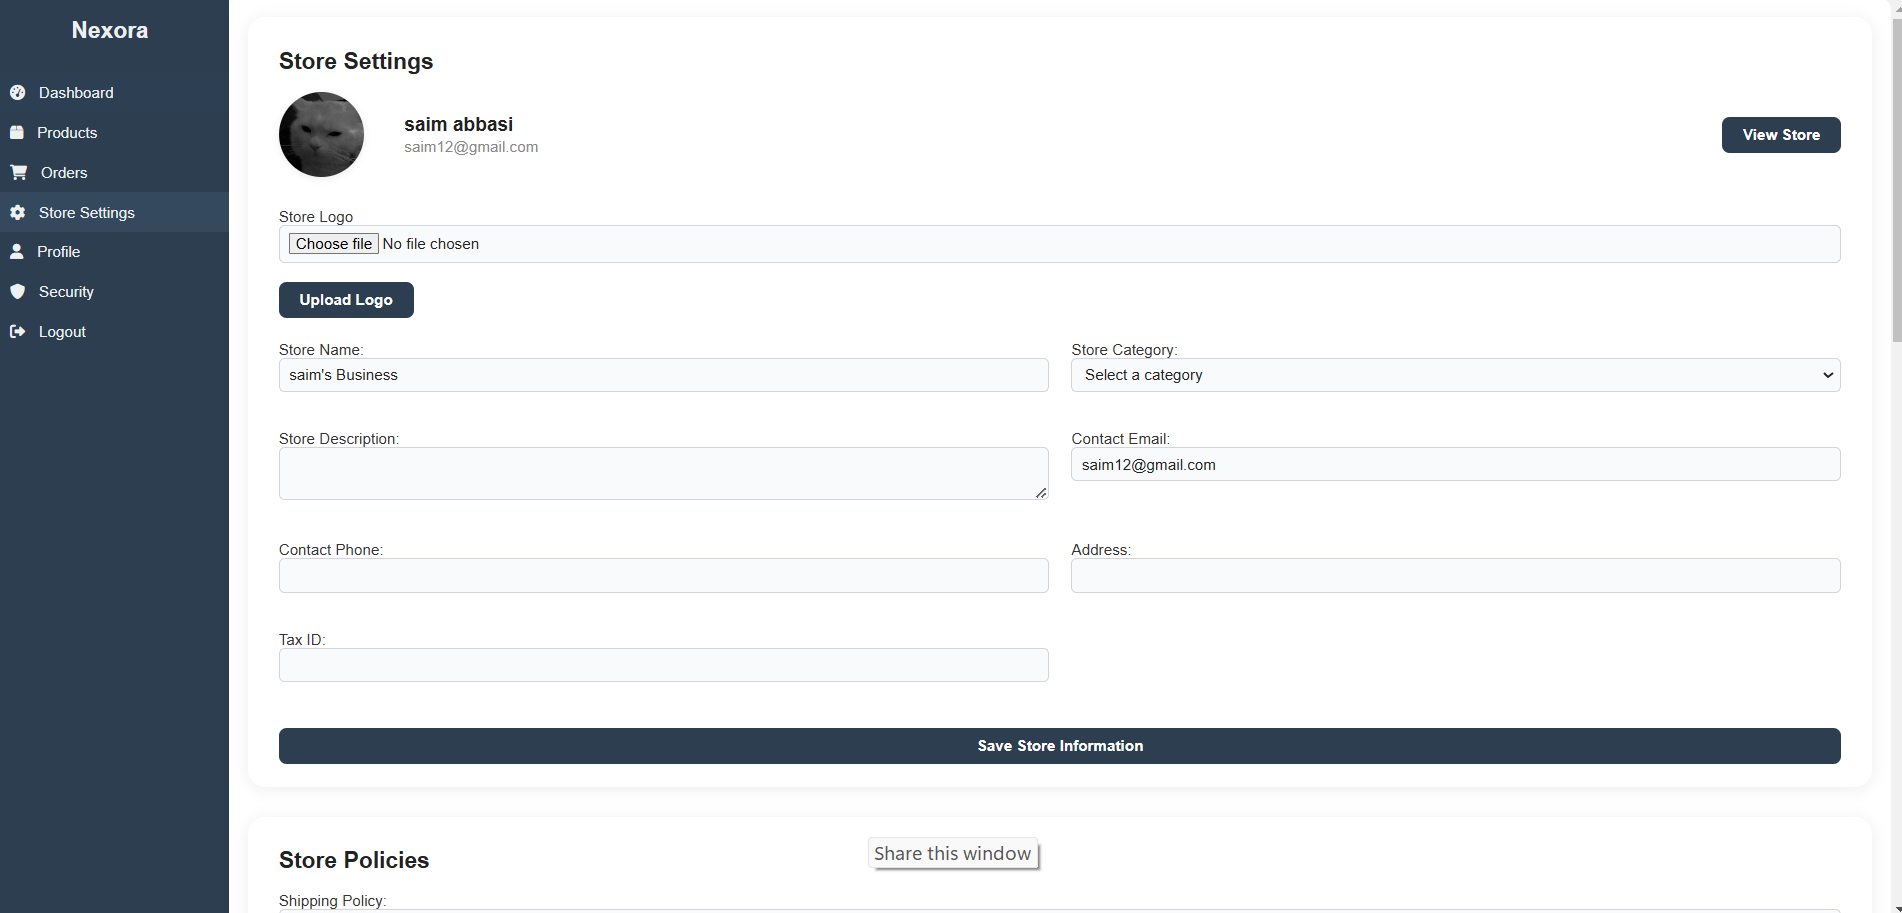
\includegraphics[width=\textwidth,keepaspectratio]{thesis/figures/vendor-store-settings.png}
\caption{Vendor Store Settings}
\label{fig:vendor-settings}
\end{figure}

% --- Admin Interface ---
\begin{figure}[htbp]
\centering
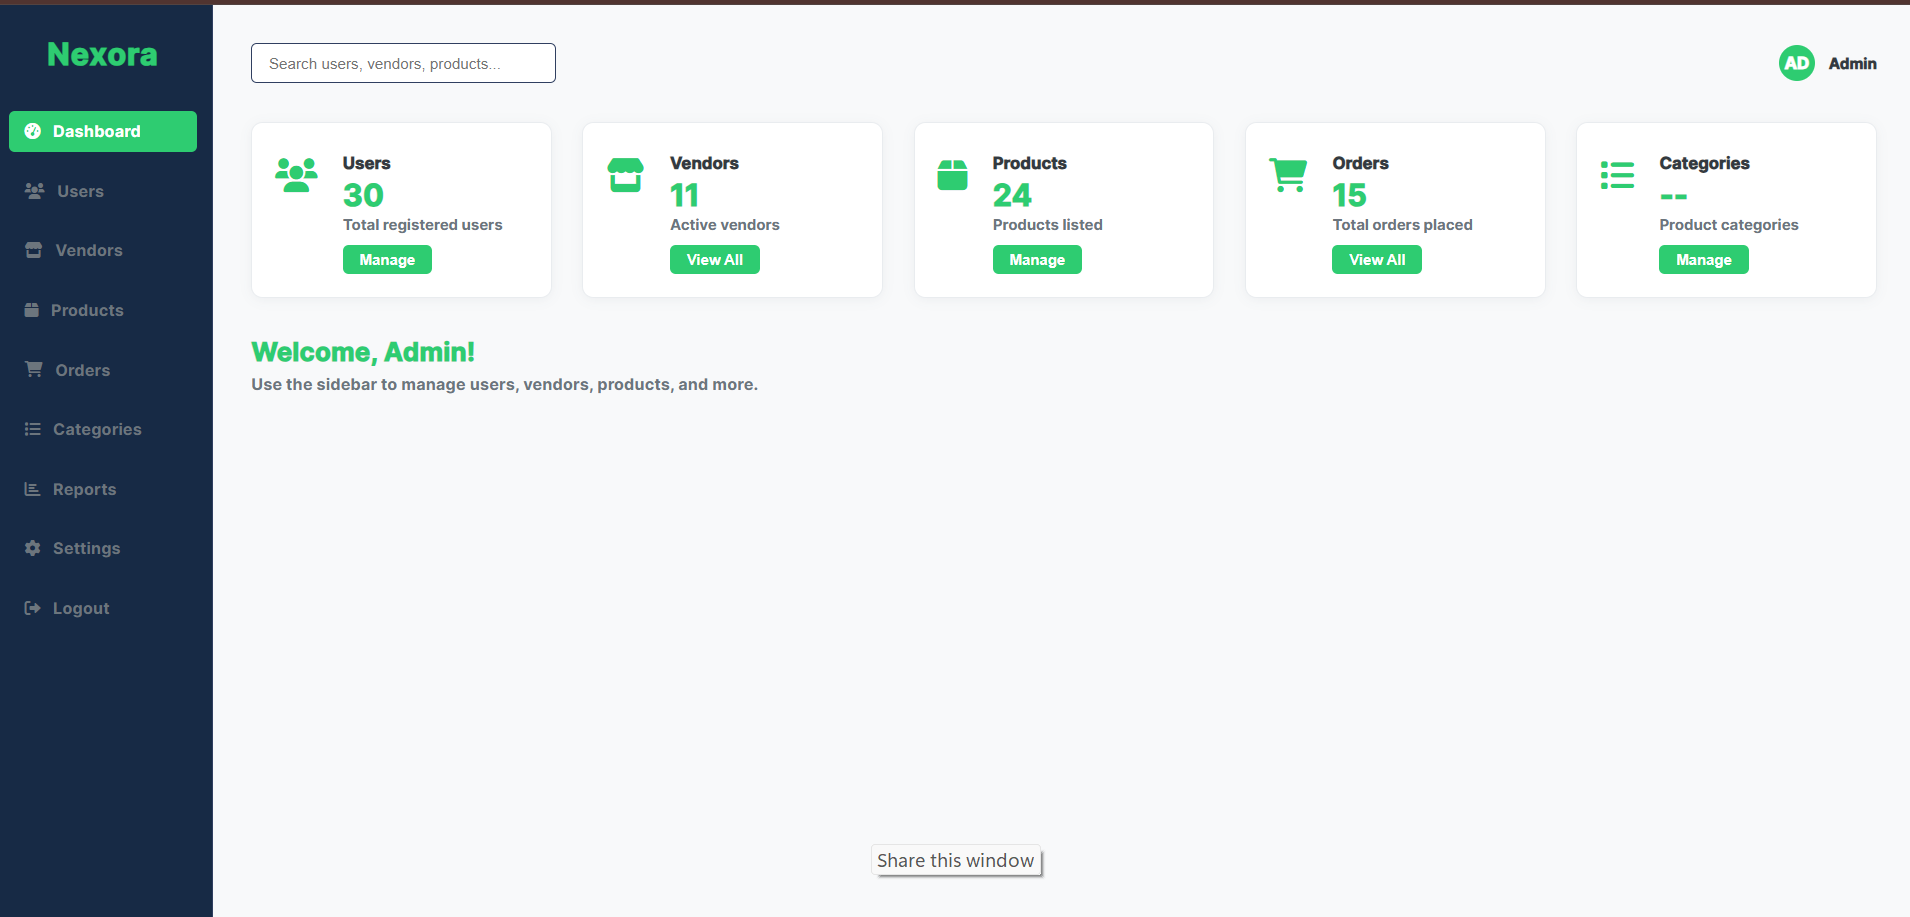
\includegraphics[width=\textwidth,keepaspectratio]{thesis/figures/admin-dashboard.png}
\caption{Admin Dashboard}
\label{fig:admin-dashboard}
\end{figure}

\begin{figure}[htbp]
\centering
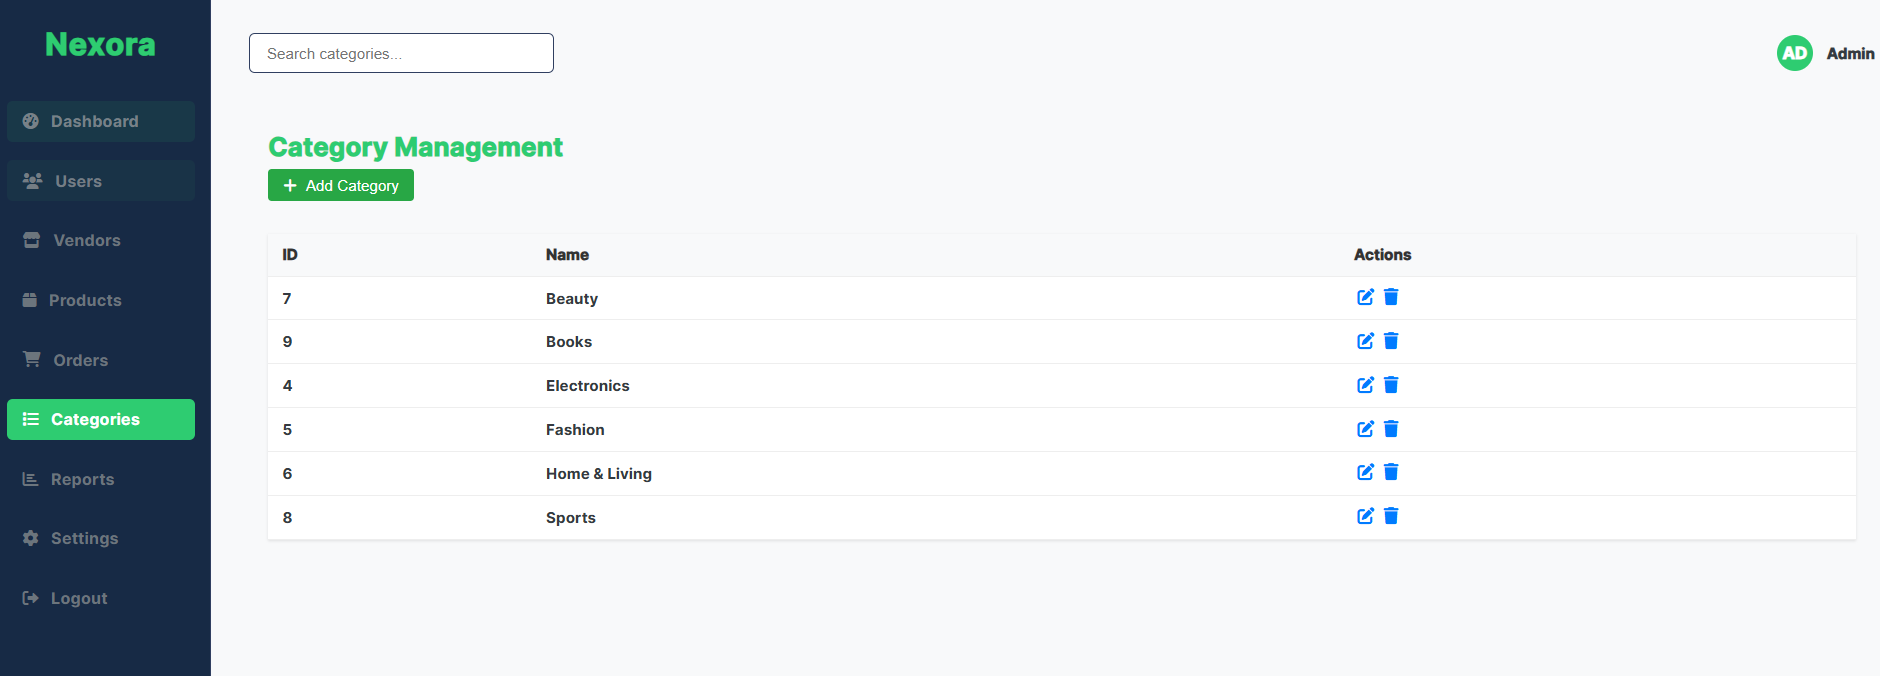
\includegraphics[width=\textwidth,keepaspectratio]{thesis/figures/admin-categories.png}
\caption{Admin Categories Management}
\label{fig:admin-categories}
\end{figure}

\begin{figure}[htbp]
\centering
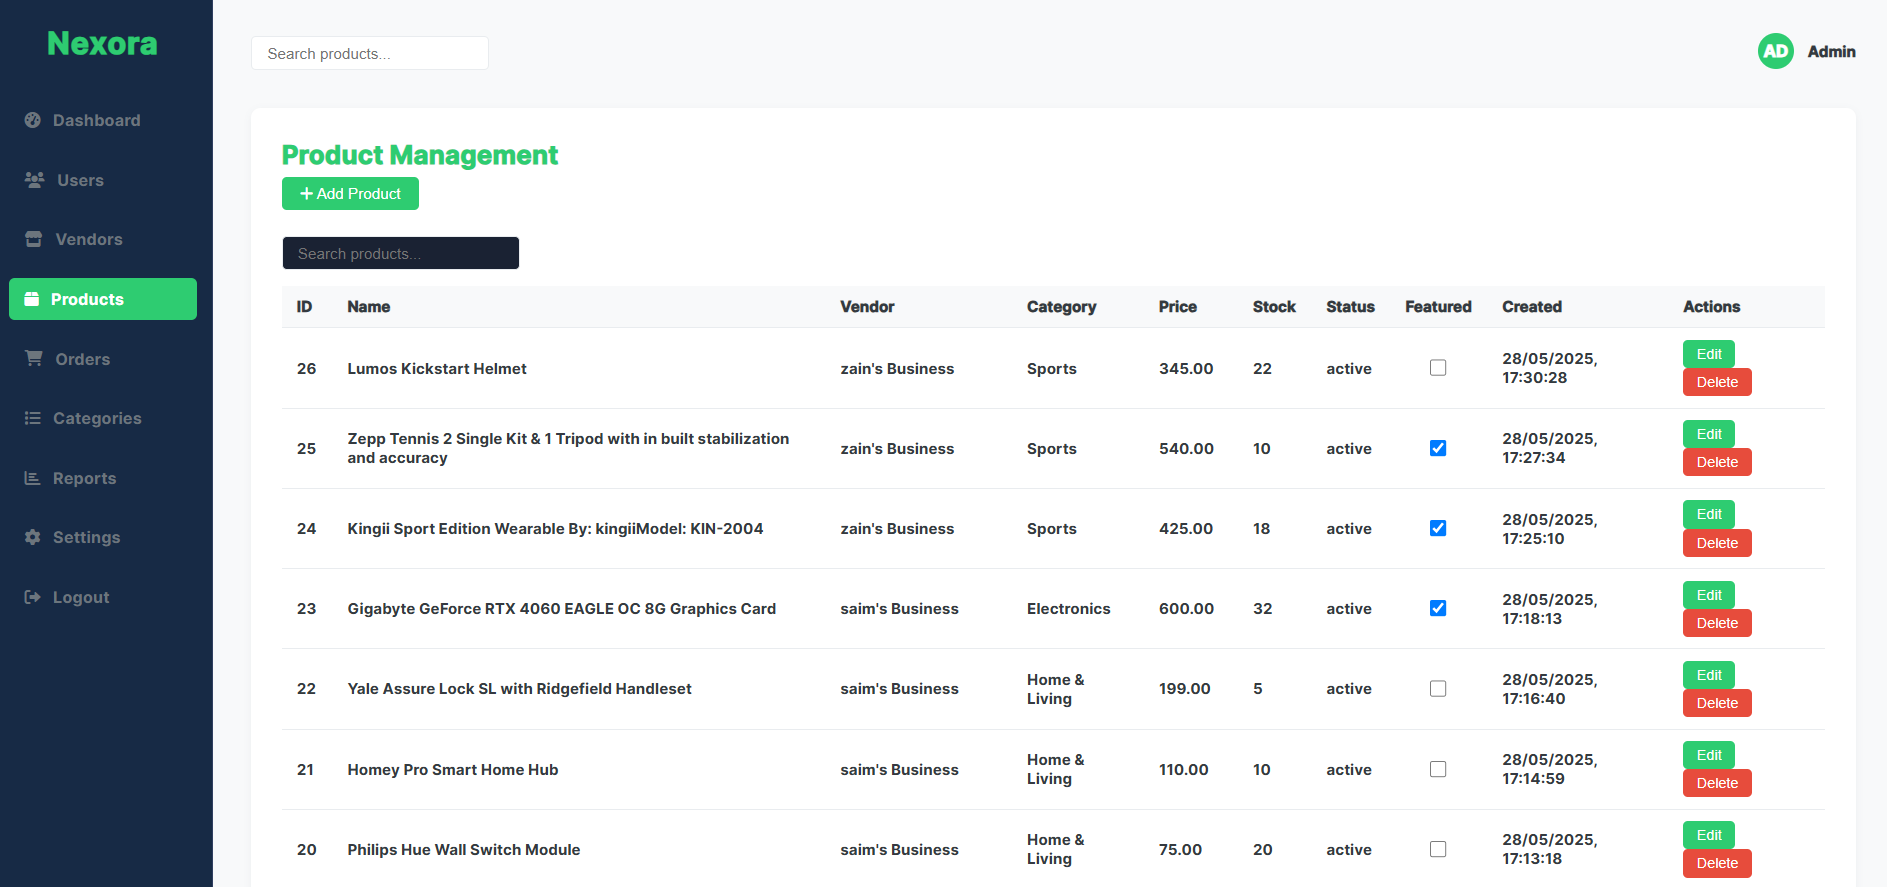
\includegraphics[width=\textwidth,keepaspectratio]{thesis/figures/admin-products-management.png}
\caption{Admin Product Management}
\label{fig:admin-products}
\end{figure}

\begin{figure}[htbp]
\centering
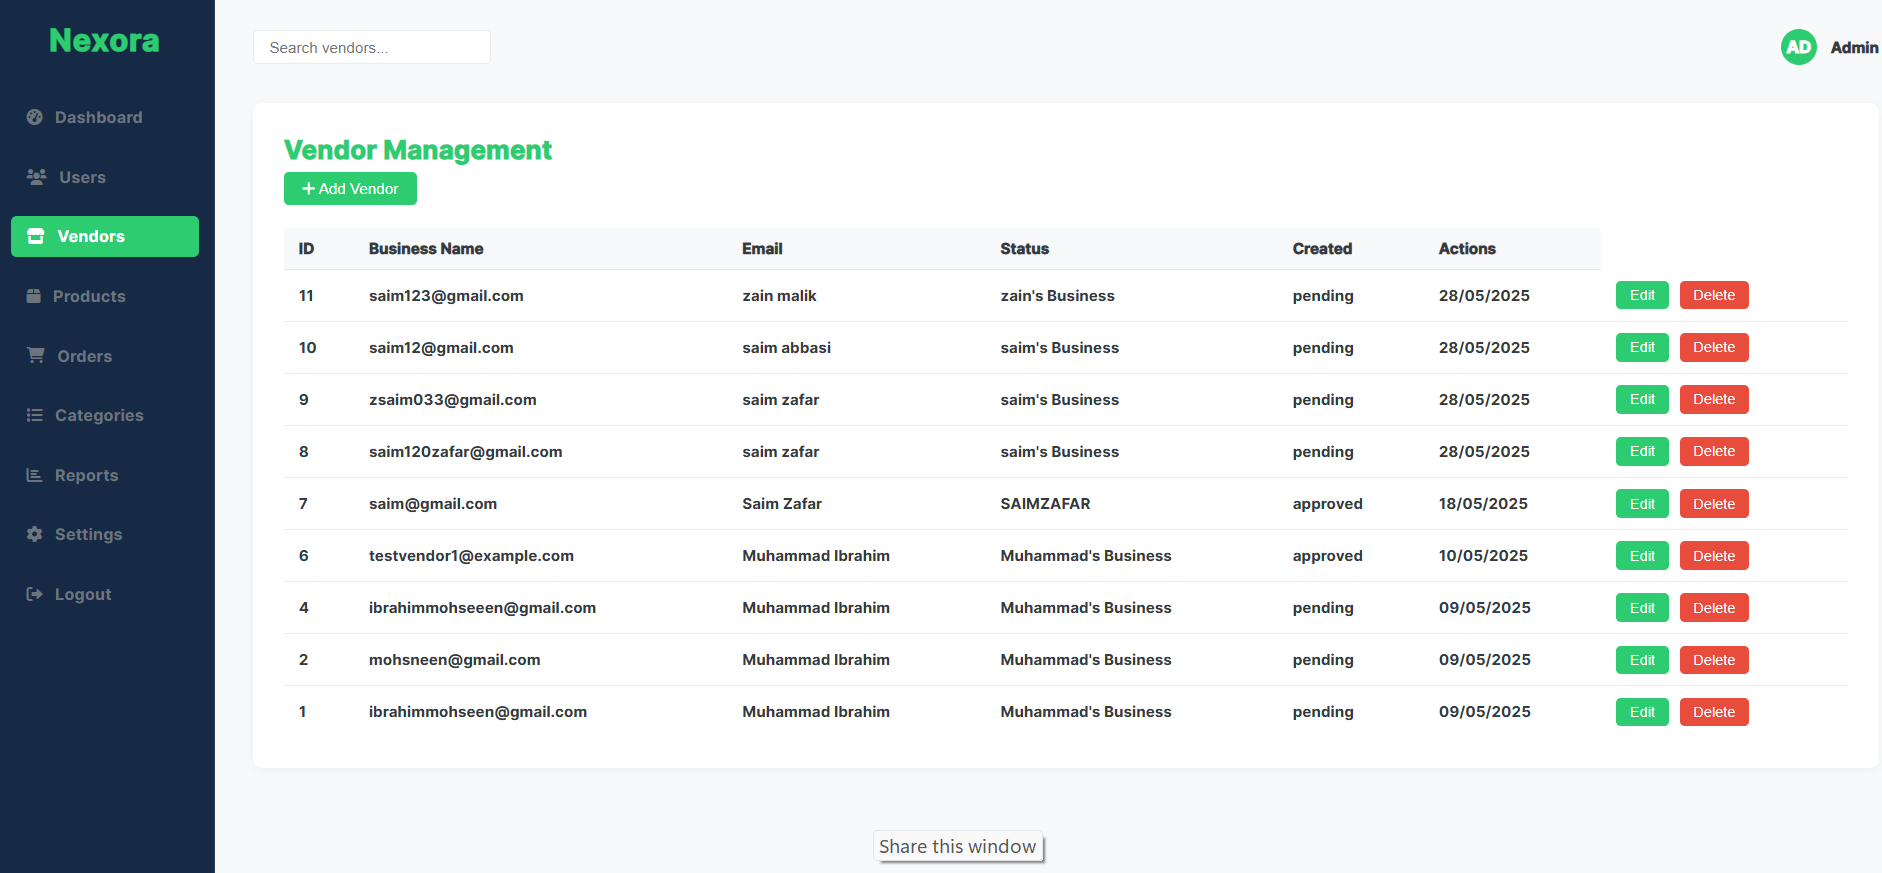
\includegraphics[width=\textwidth,keepaspectratio]{thesis/figures/admin-vendor-management.png}
\caption{Admin Vendor Management}
\label{fig:admin-vendors}
\end{figure}